\documentclass{article}

\usepackage[margin=1in]{geometry}
\usepackage[colorlinks,linkcolor=blue,filecolor=blue,citecolor=magenta,urlcolor=blue]{hyperref}
\usepackage{bm,amsmath,amsthm,amssymb,multicol,algorithmic,algorithm,enumitem,graphicx,subfigure}
\usepackage{xargs}
\usepackage{stmaryrd}


\def\M{\mathcal{M}}
\def\A{\mathcal{A}}
\def\Z{\mathcal{Z}}
\def\S{\mathcal{S}}
\def\D{\mathcal{D}}
\def\R{\mathcal{R}}
\def\P{\mathcal{P}}
\def\K{\mathcal{K}}
\def\E{\mathbb{E}}
\def\F{\mathfrak{F}}
\def\l{\boldsymbol{\ell}}

\newtheorem{Fact}{Fact}
\newtheorem{Lemma}{Lemma}
\newtheorem{Prop}{Proposition}
\newtheorem{Theorem}{Theorem} 
\newtheorem{Def}{Definition}
\newtheorem{Corollary}{Corollary}
\newtheorem{Conjecture}{Conjecture}
\newtheorem{Property}{Property}
\newtheorem{Observation}{Observation}
\newtheorem{Exa}{Example}
\newtheorem{assumption}{H\!\!}
\newtheorem{Remark}{Remark}
\newtheorem*{Lemma*}{Lemma}
\newtheorem*{Theorem*}{Theorem}
\newtheorem*{Corollary*}{Corollary}
 
\newcommand{\eqsp}{\;}
\newcommand{\beq}{\begin{equation}}
\newcommand{\eeq}{\end{equation}}
\newcommand{\eqdef}{\mathrel{\mathop:}=}
\def\EE{\mathbb{E}}
\newcommand{\norm}[1]{\left\Vert #1 \right\Vert}
\newcommand{\pscal}[2]{\left\langle#1\,|\,#2 \right\rangle}
\def\major{\mathsf{M}}
\def\rset{\ensuremath{\mathbb{R}}}


\begin{document}



\title{AniLA: Anisotropic Langevin Dynamics for training Energy-Based Models}

 \author{\textbf{Belhal Karimi, Jianwen Xie, Ping Li} \\\\
 Cognitive Computing Lab\\
 Baidu Research\\
   10900 NE 8th St. Bellevue, WA 98004, USA
 }

\date{}
\maketitle

\begin{abstract}
We develop in this paper
\end{abstract}

\section{Introduction}

Given a stream of input data noted $x$, the energy-based model (EBM) is a Gibbs distribution defined as:
\beq\label{eq:ebm}
p_{\theta}(x) = \frac{1}{Z(\theta)} \mathrm{exp}(f_{\theta}(x))
\eeq


\section{MCMC based EBM}

\paragraph{Energy Based Models: }
Energy based models \cite{lecun2006tutorial,ngiam2011learning} are a class of generative models that leverages the power of Gibbs potential and high dimensional sampling techniques to produce high quality synthetic image samples.
Training of such models occurs via Maximum Likelihood (ML).

\paragraph{MCMC procedures: }



\section{AniLA sampler based EBM}

\subsection{Preliminaries and Bottlenecks of Langevin MCMC based EBM}

\subsection{Curvature informed MCMC}

We introduce a new sampler based on the Langevin updates presented above.

\begin{algorithm}[H]
\caption{\textsc{StAnLey for Energy-Based Model}} \label{alg:anila}
\begin{algorithmic}[1]
%\small
\STATE \textbf{Input}: Total number of iterations $T$, number of MCMC transitions $K$ and of samples $M$ learning rate $\eta$, initial values $\theta_0$, $\{ z_{0}^m \}_{m=1}^M$ and $n$ observations $\{ x_{i} \}_{i=1}^n$.
\FOR{$t=1$ to $T$}
\STATE Compute the anisotropic stepsize as follows: \label{line:step}
\beq
\stepsize_t = \frac{b}{\max(b, | \nabla f_{\theta_t}(x) |}
\eeq
\STATE Draw $m$ samples $\{ z_{t}^m \}_{m=1}^M$ from the objective potential \eqref{eq:ebm} via Langevin diffusion:\label{line:langevin}
\beq
z_{t}^m = z_{t}^m + \stepsize_t/2  \nabla f_{\theta_t}(x) + \sqrt{\stepsize} \mathsf{B}_t
\eeq
where $\mathsf{B}_t$ is the brownian motion, drawn from a Normal distribution.
\STATE Samples $m$ positive observations $\{ x_{i} \}_{i=1}^m$ from the empirical data distribution
\STATE Compute the gradient of the empirical log-EBM \eqref{eq:ebm} as follows:
\beq
\nabla \sum_{i=1}^m \log p_{\theta_t}(x_i) = \mathbb{E}_{p_{\text {data }}}\left[\nabla_{\theta} f_{\theta_t}(x)\right]-\mathbb{E}_{p_{\theta}}\left[\nabla_{\theta_t} f_{\theta}(z_t^m)\right] \approx \frac{1}{m} \sum_{i=1}^{m} \nabla_{\theta} f_{\theta_t}\left(x_{i}\right)-\frac{1}{m} \sum_{i=1}^{m} \nabla_{\theta} f_{\theta_t}\left(z_t^m\right)
\eeq
\STATE Update the vector of global parameters of the EBM:
\beq
\theta_{t+1} = \theta_{t+1} + \eta \nabla \sum_{i=1}^m \log p_{\theta_t}(x_i)
\eeq
\ENDFOR
\STATE \textbf{Output:} Generated samples $\{ z_{T}^m \}_{m=1}^M$
\end{algorithmic}
\end{algorithm}



\section{Geometric ergodicity of AniLA sampler}
We will present in this section, our theoretical analysis for the Markov Chain constructed using Line~\ref{line:step}-\ref{line:langevin}. 


\section{Numerical Experiments}

\subsection{Application on Toy Example: Gaussian Mixture Model}

\begin{figure}[H]
\begin{center}
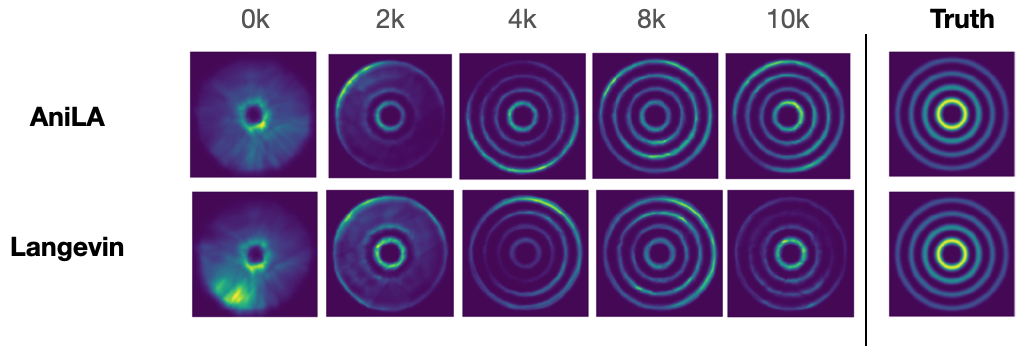
\includegraphics[width=0.8\textwidth]{figs/rings}
\caption{(Rings Toy Dataset) }
\label{fig:results}
\end{center}
\end{figure}


\subsection{Flowers Dataset}

\begin{figure}[h]
    \begin{center}
        \mbox{
        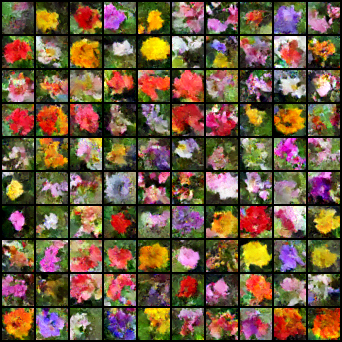
\includegraphics[width=2in]{figs/flowerslangevin}
        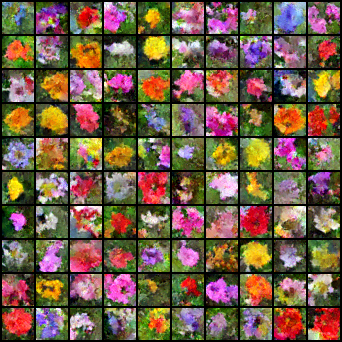
\includegraphics[width=2in]{figs/flowersanila}
        }
    \end{center}
    \vspace{-0.1in}
	\caption{(Flowers Dataset). Left: Langevin Method. Right: AniLA method. After 100k iterations.}
	\label{fig:flowers}
\end{figure}

\subsection{CIFAR Dataset}



\begin{figure}[h]
    \begin{center}
        \mbox{
        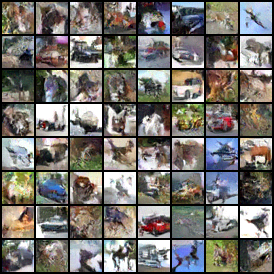
\includegraphics[width=2in]{figs/cifarlangevin}
        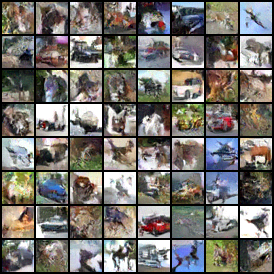
\includegraphics[width=2in]{figs/cifarlangevin}
        }
    \end{center}
    \vspace{-0.1in}
	\caption{(CIFAR Dataset). Left: Langevin Method. Right: AniLA method. After 100k iterations.}
	\label{fig:flowers}
\end{figure}

\section{Conclusion}

\newpage

\bibliographystyle{abbrvnat}
\bibliography{ref}


\end{document} 